\documentclass[french]{article}
\usepackage{amssymb, amsmath, mathtools} %pour les mathématiques
\usepackage{fontspec}
\usepackage{xunicode}
\usepackage[a4paper]{geometry}
\usepackage{babel}
\usepackage{hyperref}
\begin{document}

\title{Résumé Journalier}
\author{Joffrey Hérard}
\date{\today} 

\maketitle

\paragraph{Quels supports de VM ?}
\begin{enumerate}
	\item VirtualBox?
	\item VMWARE?
	\item LXC?
	\item Docker?
	\item QEMU?
	\item KVM?
	\item HyperV?
	\item Proxmox VE?
\end{enumerate}

\paragraph{C'est quoi faire un Test ? }
\begin{itemize}
\item Test de performance ? 
\item Test de charge ? 
\item Test de dégradations?
\item Test de robustesse ?
\item Test de montée en charge ?
\item Test aux limites?
\item Test de Benchmark ?
\end{itemize}

\paragraph{Tester quoi ?}
\begin{itemize}
	\item CPU.
	\item Disque Lecture/écriture.
	\item Transfert réseaux.
	\item Accès mémoire.
	\item GPU.  
\end{itemize}
Nécessaire d'évaluer l'impact de la virtualisation sur une même machine avec plusieurs VMs active au même moment 
\paragraph{Cas d'utilisations}
\subparagraph{Pour quel genre d'utilisateurs?}
Étant censé évaluer les performances des solutions de virtualisation d'un point de vue utilisateurs.
On ce pose la question de quoi évaluer( entrevu dans le paragraphe précédent  ), et comment (Paragraphe suivant)? Il faut faire plusieurs évaluation en fonction de quels genre d'utilisateurs on cible ? 
\begin{itemize}
	\item Un utilisateur désirant faire du HPC $\rightarrow$ Évaluations des échanges (pour les modèle a passage de message), Thread, multi-cœur.
	\item Serveurs Web $\rightarrow$ Évaluations du réseaux, évaluations des écriture/lecture disque . processeurs .
	\item etc.. 
\end{itemize}
Il faut établir des scenarios associés à chaque d'utilisations pour mettre en place une campagne de test idéal et donc en extraire des données représentatives. 
\paragraph{Driver/sans Driver ? }
\begin{itemize}
	\item Avec Driver = Installation de programme supplémentaire, meilleur performance ? pertinence ? 
	\item Sans Driver = Machine virtuelle en brute $\rightarrow$ intérêt de la virtualisation en premier lieu, créer une machines à la volée en fonction des besoins, si le besoin est immédiat le temps d'installations des drivers serait probablement trop gourmand.  
\end{itemize}
\paragraph{Ressource existante }
\subparagraph{VMWare}
	Il existe déjà un outil fournit par VMWare VMMark trouvable ici : \newline
	\url{<http://www.vmware.com/products/vmmark.html>}
\paragraph{Mis en place de test personnel ?}


\paragraph{Listes des choses à faire}
\begin{enumerate}
	\item Choix des Hyperviseurs de Type 1 ? Type 2 ? Conteneurs?
	\item Choix cible des Tests.
	\item Définitions des cas d'utilisations. 
	\item Définitions des différents scenarios associé au différent schéma ..
	\item Préparations des différents scripts associés aux scenarios pour les différent hyperviseur, conteneurs 
	\item Remise à zero de la machine hôte.
	\item Mise en place d'une << sonde >> pour effectué les relevés de sorte à être des plus neutre dans les enregistrements.
	\item Mise en place des Tests 
		\begin{enumerate}
			\item Préparations de la machine physique et des machines virtuelles. 
			\item Lancement des tests.
			\item Surveillance régulière du bon déroulement des différents test.
			\item Récupérations des données . 
			\item Analyse des résultats sur la cohérence .
			\begin{enumerate}
				\item Établir des liens entre certain paramètres $\rightarrow $ les confirmers par d'autre test ? 
				\item Analyse sur les différents hyperviseur/conteneurs sur les mêmes scenarios 
			\end{enumerate}
			\item Représentations des résultats pour chaque batterie de tests. (Courbes) et les interprétations.
			\item Retour à l’étape (a) si nécessaire sinon étapes suivantes.
		\end{enumerate}
	\item Écriture du rapport au fur et mesure.	
			
\end{enumerate}


\begin{figure}
\centering
\caption{Graphe des dépendances }
\label{Graphe des dépendances }
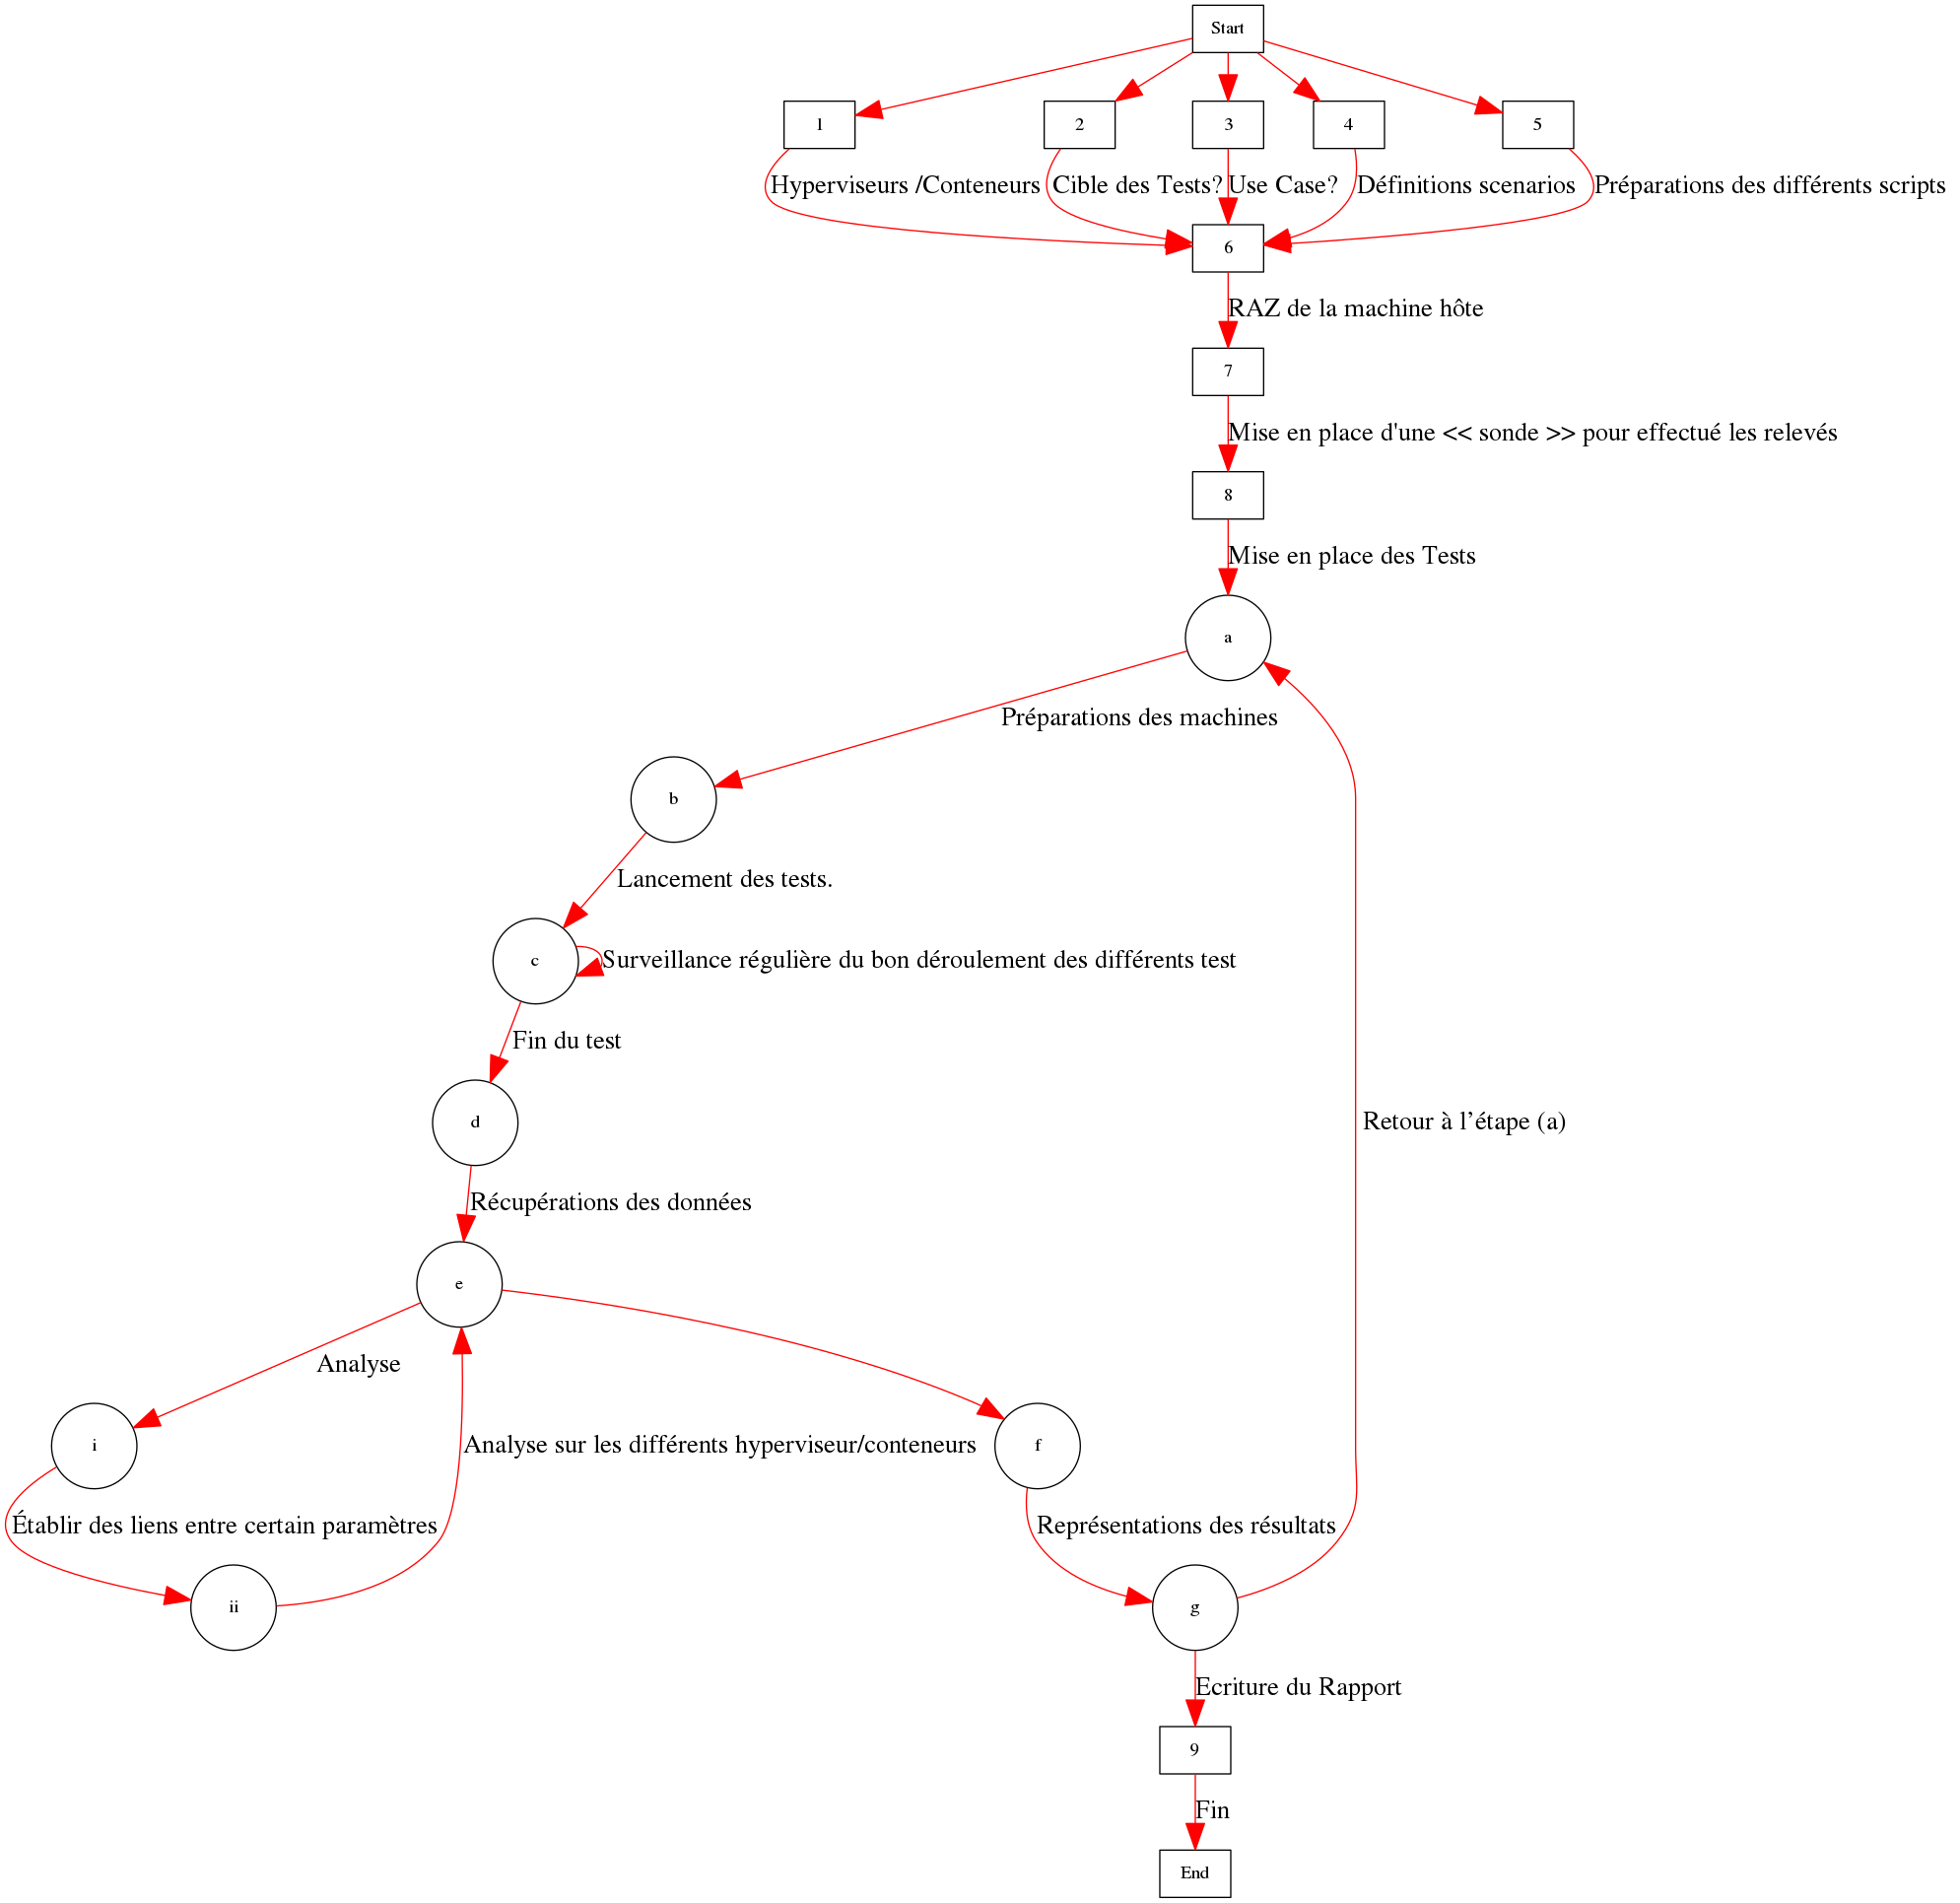
\includegraphics[scale=0.250]{GrapheDepends.png}
\end{figure}

\end{document}